\chapter{Religion, Authority, and Education I}

This chapter follows J. Krishnamurti's dialogue with Dr. Alan W. Anderson on religion, authority, and education. The source movement is not a physics lecture in the ordinary blackboard sense, and no validated board frames survive for this chapter. Still, the talk has a rigorous internal structure. We can read it as a sequence of distinctions: education and self-knowledge, religion and image, negation and reward, experience and recognition, knowledge and the living, authority and freedom. The source material is credited to J. Krishnamurti and the Krishnamurti Foundation Trust, with this course curated by LazyingArt LLC through Video2Book.

\section{Education After Death, Love, And Fear}

Anderson begins by carrying forward the previous inquiry into death in the context of living and love. The new question is education. What happens between teacher and student when they begin to look together? Why do traps, fears, and shocks appear so quickly?

Krishnamurti does not treat education as the accumulation of subjects. He asks whether education has helped us understand the actual movement of life. We may be trained for jobs, money, pleasure, social function, and religious entertainment, yet remain uneducated in the matters that most govern us: fear, pleasure, death, thought, relationship, and the sense of inward emptiness.

A compact way to put the opening charge is this:
\begin{equation}
\text{education as training}
\;\not=\;
\text{education as understanding life}.
\end{equation}

The inequality is not a formal theorem. It is a warning about misplaced emphasis. Training may be necessary, but in this dialogue it is not enough. If education leaves us unable to look at fear, death, and ourselves, then it has failed at the point where human life becomes serious.

Krishnamurti then moves almost immediately from education to religion. This is not a change of subject. Religion, as commonly lived, is one of the chief places where the uneducated mind seeks compensation for not understanding itself. If life feels empty and transient, we invent consolation. If death terrifies us, we seek permanence. If daily living has very little meaning, we create an escape and call it sacred.

\section{Religion As The Image Made By Thought}

Krishnamurti's first major construction is a genealogy of religious image-making. Human beings want to find something beyond everyday routine, beyond pleasure, beyond the daily activity of thought. But when they cannot find it directly, thought makes symbols. A stone under a tree receives marks and flowers; soon it becomes divinity. The same movement, he says, continues in cathedrals, rituals, images, chants, and worship.

The essential structure is simple enough to write as a flow:
\begin{equation}
\text{thought}
\longrightarrow
\text{image}
\longrightarrow
\text{worship of image}
\longrightarrow
\text{self-worship}.
\end{equation}

This is one of the central relations of the chapter. The mind creates the image and then bows before what it has made. The worship looks outward, but the object has been inwardly constructed. In that sense, the image is not merely an idol made by hand; it is an idolatry of the mind.

\begin{figure}
\centering
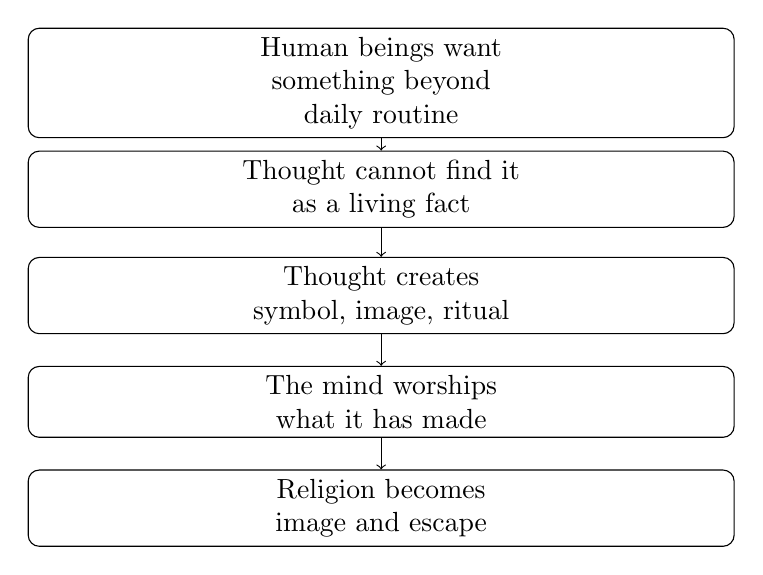
\begin{tikzpicture}
\node[draw, rounded corners, align=center, text width=0.72\linewidth] (a) at (0,0) {Human beings want\\something beyond\\daily routine};
\node[draw, rounded corners, align=center, text width=0.72\linewidth] (b) at (0,-1.35) {Thought cannot find it\\as a living fact};
\node[draw, rounded corners, align=center, text width=0.72\linewidth] (c) at (0,-2.70) {Thought creates\\symbol, image, ritual};
\node[draw, rounded corners, align=center, text width=0.72\linewidth] (d) at (0,-4.05) {The mind worships\\what it has made};
\node[draw, rounded corners, align=center, text width=0.72\linewidth] (e) at (0,-5.40) {Religion becomes\\image and escape};
\draw[->] (a) -- (b);
\draw[->] (b) -- (c);
\draw[->] (c) -- (d);
\draw[->] (d) -- (e);
\end{tikzpicture}
\caption{A transcript-derived reconstruction of the image-making sequence. No blackboard diagram was available for this lecture.}
\end{figure}

The point is not that there are many religions and therefore one must choose the right one. Krishnamurti's argument is sharper: across traditions, the same principle can operate. Thought creates an image of the Buddha, Jesus, Christ, the guru, the father, the saviour, or the ideal, and then asks that image for security.

This leads to the next question: if religion, in this sense, is image, belief, superstition, ritual, and tradition, what does it mean to negate it?

\subsection{Question \& Answer}

\paragraph{Question.}
Is negation a way of attaining something better?

\paragraph{Answer.}
Krishnamurti says no. If negation is secretly a method for gaining a better state, then it is not negation. It is still desire moving under another name. Negation, in this dialogue, means seeing what is false as false.

The distinction can be written as:
\begin{align}
\text{negation as method}
&=
\text{denial for the sake of reward},\\
\text{negation as perception}
&=
\text{seeing the false as false}.
\end{align}

Only the second meaning belongs to the lecture. The mind does not first know truth and then use that knowledge to reject error. Rather, in seeing the false clearly, the false loses its hold. Krishnamurti puts the pressure on perception itself:
\begin{equation}
\text{seeing the false as false}
\equiv
\text{negation of the false}.
\end{equation}

Again, this is not formal logic. It is a disciplined way of preserving the spoken distinction. The action is in the seeing, not in a future achievement promised by the seeing.

\section{The Tree, The Observer, And The Loss Of Direct Looking}

At this point Anderson introduces a classroom example. He had asked his students to look at a tree. One student reported an encounter that seemed clear and unblocked. Then Anderson asked whether she had been thinking of herself as looking at the tree. She hesitated. In that hesitation, she began to fall out of the act.

Krishnamurti immediately names the movement: that is the observer.

The example is crucial because it brings the earlier discussion down from religion to direct perception. The false is not only a belief or ritual. It can be the subtle self-reference that enters the act of seeing. A person may look, then form the image ``I am looking,'' then worry about giving the right report, and the direct act is already disturbed.

We can represent the sequence this way:
\begin{equation}
\text{direct looking}
\longrightarrow
\text{self-reference}
\longrightarrow
\text{hesitation}
\longrightarrow
\text{loss of direct act}.
\end{equation}

\begin{proposition}
In the classroom example, the observer is not a separate entity discovered behind perception. It is the movement of self-reference entering perception.
\end{proposition}

\begin{proof}
We follow the order of the example.
\begin{enumerate}
\item The student first describes looking at the tree without obvious blockage.
\item The question is raised: was she thinking of herself as looking?
\item The act becomes self-conscious.
\item She begins to worry about saying the right thing in class.
\item The original relation to the tree is displaced by the image of herself as the one who must report correctly.
\end{enumerate}
Thus the observer is not added as a theory. It is observed in the very movement from looking to self-reference.
\end{proof}

This is also why the classroom scene belongs inside the inquiry into education. Education is not merely the transmission of facts. It is tested at the point where a student looks, hesitates, becomes self-conscious, and asks whether inquiry can continue without fear of authority, performance, or correctness.

\section{Experience, Recognition, And The Old}

Krishnamurti next says that one must go much more deeply into thought. Thought has created the technological world, but it has also created religions, chants, cathedrals, images, masters, gurus, and father figures. Unless thought is understood, the same pattern repeats in another field.

Anderson then introduces the word ``experience.'' People say they need the experience of awakening, the experience of God, the experience of something outside themselves. Krishnamurti asks why this demand for experience arises at all. We already have experiences of every kind: insult, flattery, incident, influence, pleasure, frustration. But we become bored with ordinary experience and want a special one.

The key argument is exact enough to state as a worked derivation.

\subsection{Question \& Answer}

\paragraph{Question.}
Can an experience be genuinely new if it is recognized as an experience?

\paragraph{Answer.}
Krishnamurti's answer is no. If I know that I have had an experience, I have recognized it. Recognition implies that I already know what I am recognizing. Therefore the so-called new experience is tied to the old.

\begin{proposition}
A recognized ``new'' spiritual experience is not new in Krishnamurti's sense.
\end{proposition}

\begin{proof}
Let us keep the reasoning in the order of the dialogue.
\begin{enumerate}
\item I say that I have had an experience.
\item To say this, I must know that the experience has occurred.
\item To know that it has occurred, I must recognize it.
\item Recognition depends on what is already known.
\item Therefore the experience, insofar as it is recognized, belongs to the field of the already known.
\item What belongs to the already known is not the new.
\end{enumerate}
So the claim to possess a new spiritual experience collapses back into memory, recognition, and self-deception.
\end{proof}

The compressed relation is:
\begin{equation}
\text{experience known as experience}
\longrightarrow
\text{recognition}
\longrightarrow
\text{already known}
\longrightarrow
\text{not new}.
\end{equation}

This is the most formal part of the lecture's reasoning. It should not be overstated as a general theory of experience. It is aimed at the religious demand for a special experience, especially when that experience is promised by someone who claims to possess knowledge.

\section{Beauty Or Gratification Through Beauty}

The discussion of experience leads Anderson to chant, cadence, and beauty. He mentions Sanskrit invocation and the possibility that beautiful words can bring euphoria or somnolence. The question is not whether chant, architecture, music, robes, incense, or colored light are ugly. The question is whether beauty becomes another trap when the self seeks gratification through it.

Krishnamurti's distinction can be written as:
\begin{align}
\text{beauty}
&\sim
\text{emptying of self},\\
\text{gratification through beauty}
&\sim
\text{satisfaction, relief, sacred feeling}.
\end{align}

The second line is what religious atmosphere often supplies. A person enters a cathedral, hears music, sees colored light, smells incense, and feels quiet, happy, relieved, perhaps in contact with something. Krishnamurti's objection is not to color, sound, or form as such. It is to mistaking the satisfaction they produce for transformation in daily life.

This passage must be paced carefully. If we reduce it to an attack on music or architecture, we miss the point. Anderson himself warns against blaming the music, as though the music were the seducer and not the self. Krishnamurti agrees with that direction. The trap is the self seeking continuity, relief, and sacred feeling through beauty.

A compact table preserves the distinction:

\begin{table}
\centering
\begin{tabular}{p{0.42\linewidth} p{0.42\linewidth}}
\hline
Beauty without self & Gratification through beauty \\
\hline
Abandonment of the self & Satisfaction of the self \\
Emptying of consciousness of its content & Relief through words, robes, incense, architecture \\
Not dependent on religious trappings & Often mistaken for sacredness \\
Bears on how one lives & Can remain separate from daily life \\
\hline
\end{tabular}
\caption{A compact reconstruction of the lecture's distinction between beauty and gratification through beauty.}
\end{table}

Krishnamurti then condenses the matter: experience is a trap. The word ``knowledge'' now enters. People who want strange experience often call it knowledge, and those who claim to have it offer it to others.

\section{Knowledge, Authority, And The Intermediary}

The inquiry turns from experience to knowledge. Krishnamurti asks what a person means by saying, ``I know,'' especially in spiritual matters. What is known, he says, is something past, finished, dead. A living thing is moving and never the same. Therefore one cannot truly say, in this possessive sense, ``I know'' a living human being.

The relation is:
\begin{equation}
\text{knowledge}
\sim
\text{the past},
\qquad
\text{the living}
\not\sim
\text{known possession}.
\end{equation}

This is not anti-intellectualism. It is directed at the claim of spiritual possession: I know, I have experienced, I have knowledge, and I will give it to you. Krishnamurti calls this impudence because it turns the living into the already known and then asks others to obey.

From here the lecture moves to authority. There is practical authority: traffic laws, the side of the road, the doctor's advice heard carefully and watchfully. But there is also inward authority: the priest, guru, spiritual leader, or intermediary who claims to know what the seeker does not.

\begin{table}
\centering
\begin{tabular}{p{0.42\linewidth} p{0.42\linewidth}}
\hline
Practical authority & Inward authority \\
\hline
Law, road rules, practical order & Priest, guru, intermediary \\
Can be listened to watchfully & Often accepted through fear or despair \\
Does not require inward slavery & Claims spiritual knowledge or protection \\
Belongs to functional life & Invades freedom, intelligence, and inquiry \\
\hline
\end{tabular}
\caption{The lecture's distinction between practical authority and inward authority.}
\end{table}

Krishnamurti asks why a mind that rejects political tyranny may accept spiritual tyranny. The answer is not supplied as a slogan. He circles through fear, despair, loneliness, ignorance, the wish for comfort, the wish to be protected, and the longing for someone else to do the inward work.

The chain is:
\begin{equation}
\text{fear, loneliness, ignorance}
\longrightarrow
\text{acceptance of authority}
\longrightarrow
\text{obedience}
\longrightarrow
\text{loss of inward freedom}.
\end{equation}

Anderson sharpens the matter by recalling the infant's need. The infant has a radical need: food, holding, protection. There is no intermediary of its own contrivance. Later, as one grows older, thought begins to imagine the source of the meeting of need. An image is inserted between danger and action.

We should state this cautiously, since it is Anderson's formulation and Krishnamurti agrees to it. The contrast is:
\begin{align}
\text{radical need}
&\longrightarrow
\text{immediate action},\\
\text{sense of danger}
&\longrightarrow
\text{image or intermediary}
\longrightarrow
\text{deferred action}.
\end{align}

The diagram below keeps the contrast narrow enough for pocket layout.

\begin{figure}
\centering
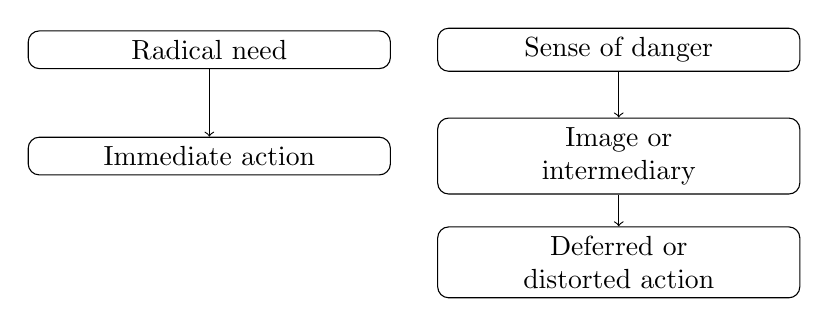
\begin{tikzpicture}
\node[draw, rounded corners, align=center, text width=0.36\linewidth] (a) at (-2.6,0) {Radical need};
\node[draw, rounded corners, align=center, text width=0.36\linewidth] (b) at (-2.6,-1.35) {Immediate action};

\node[draw, rounded corners, align=center, text width=0.36\linewidth] (c) at (2.6,0) {Sense of danger};
\node[draw, rounded corners, align=center, text width=0.36\linewidth] (d) at (2.6,-1.35) {Image or\\intermediary};
\node[draw, rounded corners, align=center, text width=0.36\linewidth] (e) at (2.6,-2.70) {Deferred or\\distorted action};

\draw[->] (a) -- (b);
\draw[->] (c) -- (d);
\draw[->] (d) -- (e);
\end{tikzpicture}
\caption{A cautious reconstruction of Anderson's contrast between immediate need and the later insertion of image or intermediary.}
\end{figure}

The practical payoff is severe: inwardly we may stop reasoning exactly where freedom, intelligence, and reasoning are most needed. Someone tells us what to do, and we repeat. Tradition, repetition, discipline, and obedience then replace inquiry.

\section{Education Without Authority}

The last movement returns to education. If current education trains thought, memory, acceptance, obedience, and reaction, can there be an education in which there is no psychological authority whatsoever?

\subsection{Question \& Answer}

\paragraph{Question.}
Can there be education without authority?

\paragraph{Answer.}
The dialogue does not close the question with a system. Anderson says yes, drawing on his classroom experience, but the yes is experimental, not institutional. He describes students shocked by the invitation to work together: not to do what the teacher says, but to question together.

This is the educational form of the whole lecture. The teacher is not the one who knows and gives knowledge to the ignorant. The teacher and student share inquiry. But this immediately exposes another difficulty: students who have been trained to try, obey, perform, and succeed may freeze when authority is suspended.

The movement can be expressed as:
\begin{equation}
\text{authority-free inquiry}
\longrightarrow
\text{shock}
\longrightarrow
\text{attention}
\longrightarrow
\text{hesitation}.
\end{equation}

Anderson calls this moment decisive. The students stand at the edge of an abyss; the water reaches the lip of the cup and cannot quite spill over. Krishnamurti replies from long experience with schools: when students are asked about freedom, authority, and acceptance, they are often lost. They want slavery, or they reject slavery in one form while accepting it in another.

The lecture therefore ends unfinished by design. The final question is not merely how to found a school. It is whether the mind can learn without inward authority, without turning the teacher into an intermediary, without converting attention into effort, and without freezing at the first glimpse of freedom.

\section{Summary}

The chapter's movement is continuous. Education is questioned because it has not taught us to understand life. Religion is questioned because thought creates images and then seeks security in them. Negation is clarified as seeing the false, not pursuing reward. Anderson's tree example shows the observer entering the act of looking. The demand for experience is examined through recognition: what is recognized is already known, and therefore not new. Beauty is distinguished from gratification through beauty. Knowledge is questioned where it claims possession of the living. Authority is traced to fear, loneliness, ignorance, repetition, and the wish for someone else to do the inward work.

The final educational question remains open:
\begin{equation}
\text{Can teacher and student inquire together}
\quad
\text{without psychological authority?}
\end{equation}

That question carries the lecture forward. It belongs to Part III of the wider inquiry because it turns toward attention, freedom, education, and transformation, while still carrying the earlier investigations of fear, death, desire, image, and relationship inside it.